\documentclass[1p]{elsarticle_modified}
%\bibliographystyle{elsarticle-num}

%\usepackage[colorlinks]{hyperref}
%\usepackage{abbrmath_seonhwa} %\Abb, \Ascr, \Acal ,\Abf, \Afrak
\usepackage{amsfonts}
\usepackage{amssymb}
\usepackage{amsmath}
\usepackage{amsthm}
\usepackage{scalefnt}
\usepackage{amsbsy}
\usepackage{kotex}
\usepackage{caption}
\usepackage{subfig}
\usepackage{color}
\usepackage{graphicx}
\usepackage{xcolor} %% white, black, red, green, blue, cyan, magenta, yellow
\usepackage{float}
\usepackage{setspace}
\usepackage{hyperref}

\usepackage{tikz}
\usetikzlibrary{arrows}

\usepackage{multirow}
\usepackage{array} % fixed length table
\usepackage{hhline}

%%%%%%%%%%%%%%%%%%%%%
\makeatletter
\renewcommand*\env@matrix[1][\arraystretch]{%
	\edef\arraystretch{#1}%
	\hskip -\arraycolsep
	\let\@ifnextchar\new@ifnextchar
	\array{*\c@MaxMatrixCols c}}
\makeatother %https://tex.stackexchange.com/questions/14071/how-can-i-increase-the-line-spacing-in-a-matrix
%%%%%%%%%%%%%%%

\usepackage[normalem]{ulem}

\newcommand{\msout}[1]{\ifmmode\text{\sout{\ensuremath{#1}}}\else\sout{#1}\fi}
%SOURCE: \msout is \stkout macro in https://tex.stackexchange.com/questions/20609/strikeout-in-math-mode

\newcommand{\cancel}[1]{
	\ifmmode
	{\color{red}\msout{#1}}
	\else
	{\color{red}\sout{#1}}
	\fi
}

\newcommand{\add}[1]{
	{\color{blue}\uwave{#1}}
}

\newcommand{\replace}[2]{
	\ifmmode
	{\color{red}\msout{#1}}{\color{blue}\uwave{#2}}
	\else
	{\color{red}\sout{#1}}{\color{blue}\uwave{#2}}
	\fi
}

\newcommand{\Sol}{\mathcal{S}} %segment
\newcommand{\D}{D} %diagram
\newcommand{\A}{\mathcal{A}} %arc


%%%%%%%%%%%%%%%%%%%%%%%%%%%%%5 test

\def\sl{\operatorname{\textup{SL}}(2,\Cbb)}
\def\psl{\operatorname{\textup{PSL}}(2,\Cbb)}
\def\quan{\mkern 1mu \triangleright \mkern 1mu}

\theoremstyle{definition}
\newtheorem{thm}{Theorem}[section]
\newtheorem{prop}[thm]{Proposition}
\newtheorem{lem}[thm]{Lemma}
\newtheorem{ques}[thm]{Question}
\newtheorem{cor}[thm]{Corollary}
\newtheorem{defn}[thm]{Definition}
\newtheorem{exam}[thm]{Example}
\newtheorem{rmk}[thm]{Remark}
\newtheorem{alg}[thm]{Algorithm}

\newcommand{\I}{\sqrt{-1}}
\begin{document}

%\begin{frontmatter}
%
%\title{Boundary parabolic representations of knots up to 8 crossings}
%
%%% Group authors per affiliation:
%\author{Yunhi Cho} 
%\address{Department of Mathematics, University of Seoul, Seoul, Korea}
%\ead{yhcho@uos.ac.kr}
%
%
%\author{Seonhwa Kim} %\fnref{s_kim}}
%\address{Center for Geometry and Physics, Institute for Basic Science, Pohang, 37673, Korea}
%\ead{ryeona17@ibs.re.kr}
%
%\author{Hyuk Kim}
%\address{Department of Mathematical Sciences, Seoul National University, Seoul 08826, Korea}
%\ead{hyukkim@snu.ac.kr}
%
%\author{Seokbeom Yoon}
%\address{Department of Mathematical Sciences, Seoul National University, Seoul, 08826,  Korea}
%\ead{sbyoon15@snu.ac.kr}
%
%\begin{abstract}
%We find all boundary parabolic representation of knots up to 8 crossings.
%
%\end{abstract}
%\begin{keyword}
%    \MSC[2010] 57M25 
%\end{keyword}
%
%\end{frontmatter}

%\linenumbers
%\tableofcontents
%
\newcommand\colored[1]{\textcolor{white}{\rule[-0.35ex]{0.8em}{1.4ex}}\kern-0.8em\color{red} #1}%
%\newcommand\colored[1]{\textcolor{white}{ #1}\kern-2.17ex	\textcolor{white}{ #1}\kern-1.81ex	\textcolor{white}{ #1}\kern-2.15ex\color{red}#1	}

{\Large $\underline{11n_{21}~(K11n_{21})}$}

\setlength{\tabcolsep}{10pt}
\renewcommand{\arraystretch}{1.6}
\vspace{1cm}\begin{tabular}{m{100pt}>{\centering\arraybackslash}m{274pt}}
\multirow{5}{120pt}{
	\centering
	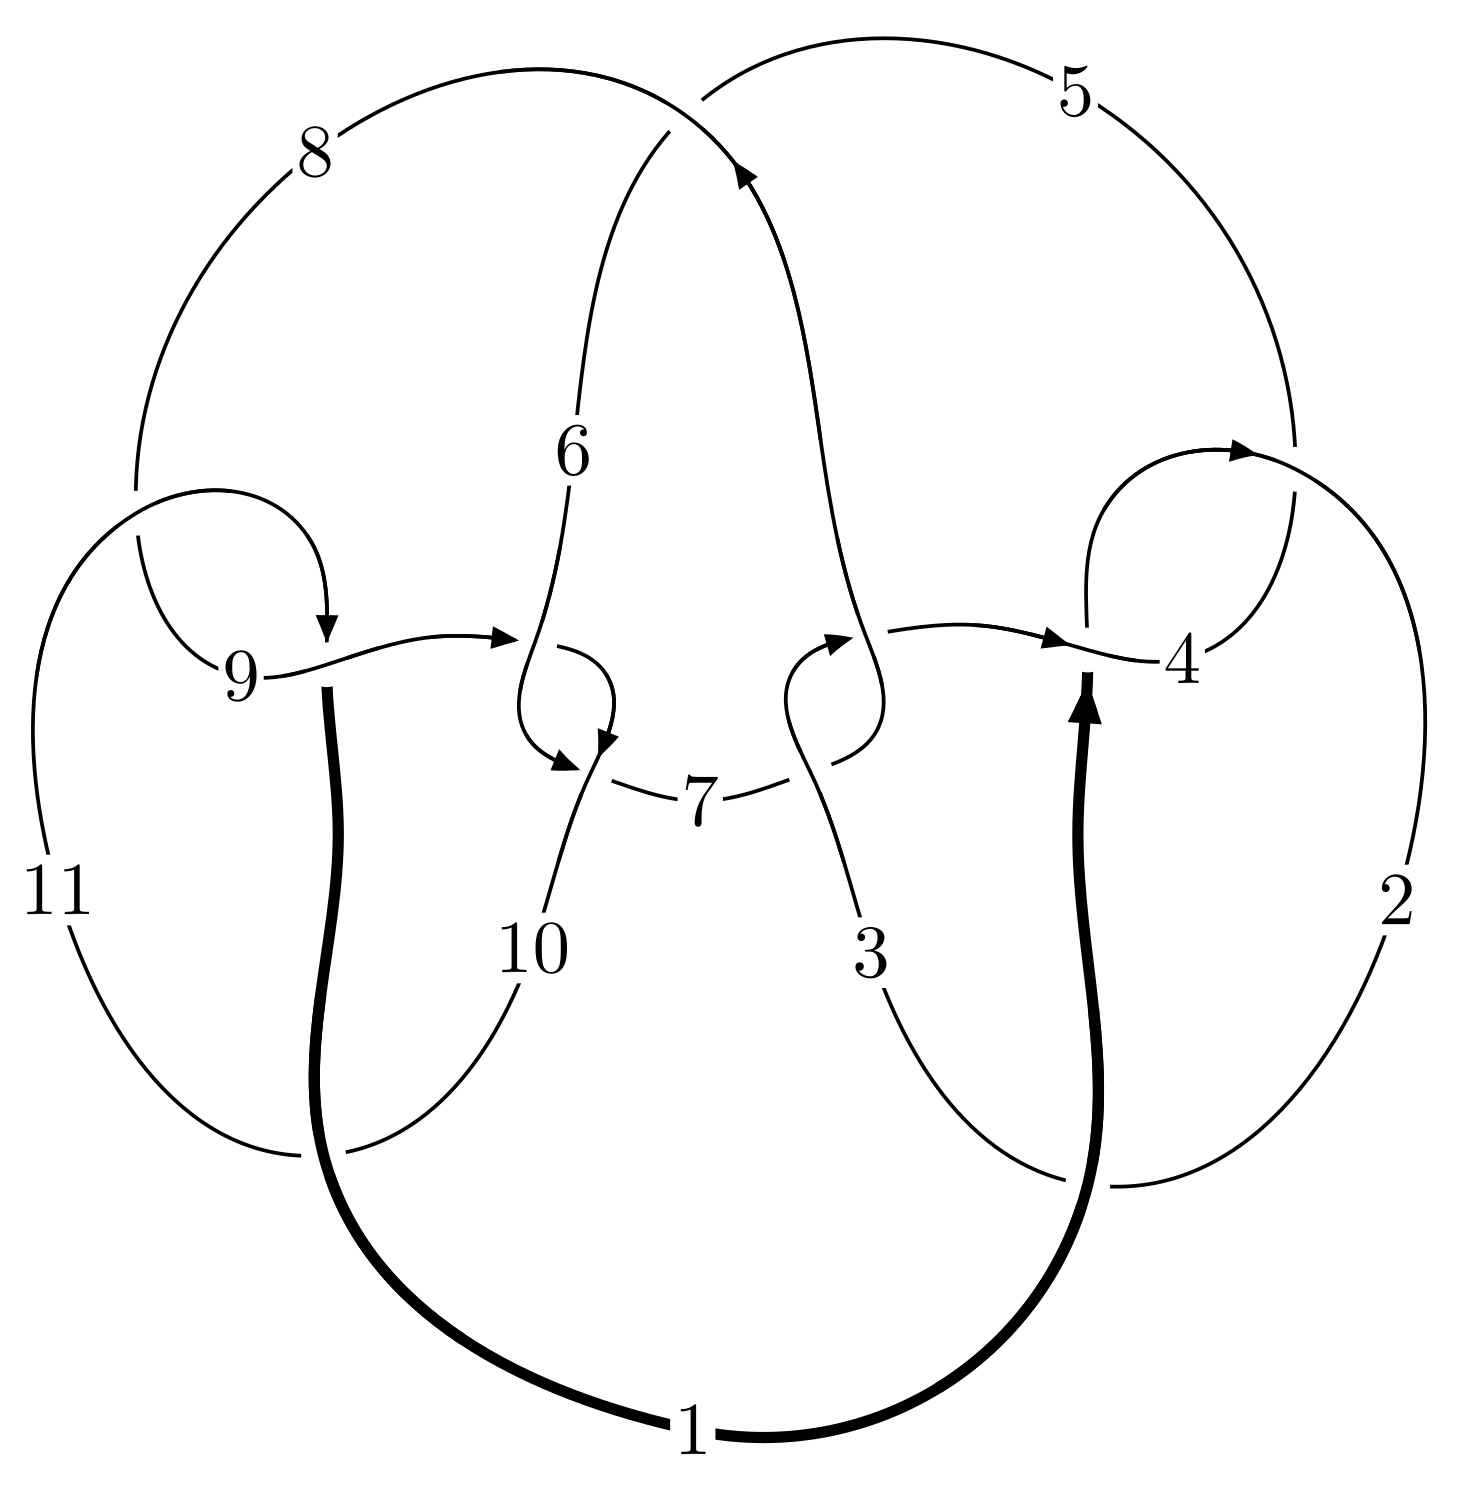
\includegraphics[width=112pt]{../../../GIT/diagram.site/Diagrams/png/637_11n_21.png}\\
\ \ \ A knot diagram\footnotemark}&
\allowdisplaybreaks
\textbf{Linearized knot diagam} \\
\cline{2-2}
 &
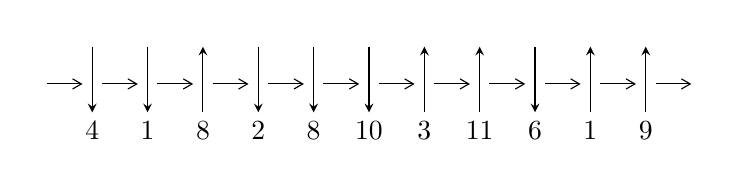
\begin{tikzpicture}[x=20pt, y=17pt]
	% nodes
	\node (C0) at (0, 0) {};
	\node (C1) at (1, 0) {};
	\node (C1U) at (1, +1) {};
	\node (C1D) at (1, -1) {4};

	\node (C2) at (2, 0) {};
	\node (C2U) at (2, +1) {};
	\node (C2D) at (2, -1) {1};

	\node (C3) at (3, 0) {};
	\node (C3U) at (3, +1) {};
	\node (C3D) at (3, -1) {8};

	\node (C4) at (4, 0) {};
	\node (C4U) at (4, +1) {};
	\node (C4D) at (4, -1) {2};

	\node (C5) at (5, 0) {};
	\node (C5U) at (5, +1) {};
	\node (C5D) at (5, -1) {8};

	\node (C6) at (6, 0) {};
	\node (C6U) at (6, +1) {};
	\node (C6D) at (6, -1) {10};

	\node (C7) at (7, 0) {};
	\node (C7U) at (7, +1) {};
	\node (C7D) at (7, -1) {3};

	\node (C8) at (8, 0) {};
	\node (C8U) at (8, +1) {};
	\node (C8D) at (8, -1) {11};

	\node (C9) at (9, 0) {};
	\node (C9U) at (9, +1) {};
	\node (C9D) at (9, -1) {6};

	\node (C10) at (10, 0) {};
	\node (C10U) at (10, +1) {};
	\node (C10D) at (10, -1) {1};

	\node (C11) at (11, 0) {};
	\node (C11U) at (11, +1) {};
	\node (C11D) at (11, -1) {9};
	\node (C12) at (12, 0) {};

	% arrows
	\draw[->,>={angle 60}]
	(C0) edge (C1) (C1) edge (C2) (C2) edge (C3) (C3) edge (C4) (C4) edge (C5) (C5) edge (C6) (C6) edge (C7) (C7) edge (C8) (C8) edge (C9) (C9) edge (C10) (C10) edge (C11) (C11) edge (C12) ;	\draw[->,>=stealth]
	(C1U) edge (C1D) (C2U) edge (C2D) (C3D) edge (C3U) (C4U) edge (C4D) (C5U) edge (C5D) (C6U) edge (C6D) (C7D) edge (C7U) (C8D) edge (C8U) (C9U) edge (C9D) (C10D) edge (C10U) (C11D) edge (C11U) ;
	\end{tikzpicture} \\
\hhline{~~} \\& 
\textbf{Solving Sequence} \\ \cline{2-2} 
 &
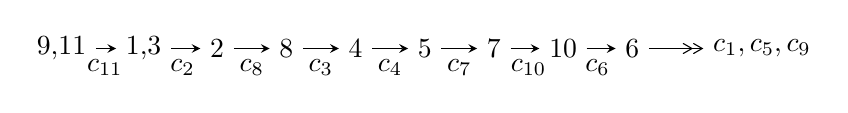
\begin{tikzpicture}[x=25pt, y=7pt]
	% node
	\node (A0) at (-1/8, 0) {9,11};
	\node (A1) at (17/16, 0) {1,3};
	\node (A2) at (17/8, 0) {2};
	\node (A3) at (25/8, 0) {8};
	\node (A4) at (33/8, 0) {4};
	\node (A5) at (41/8, 0) {5};
	\node (A6) at (49/8, 0) {7};
	\node (A7) at (57/8, 0) {10};
	\node (A8) at (65/8, 0) {6};
	\node (C1) at (1/2, -1) {$c_{11}$};
	\node (C2) at (13/8, -1) {$c_{2}$};
	\node (C3) at (21/8, -1) {$c_{8}$};
	\node (C4) at (29/8, -1) {$c_{3}$};
	\node (C5) at (37/8, -1) {$c_{4}$};
	\node (C6) at (45/8, -1) {$c_{7}$};
	\node (C7) at (53/8, -1) {$c_{10}$};
	\node (C8) at (61/8, -1) {$c_{6}$};
	\node (A9) at (10, 0) {$c_{1},c_{5},c_{9}$};

	% edge
	\draw[->,>=stealth]	
	(A0) edge (A1) (A1) edge (A2) (A2) edge (A3) (A3) edge (A4) (A4) edge (A5) (A5) edge (A6) (A6) edge (A7) (A7) edge (A8) ;
	\draw[->>,>={angle 60}]	
	(A8) edge (A9);
\end{tikzpicture} \\ 

\end{tabular} \\

\footnotetext{
The image of knot diagram is generated by the software ``\textbf{Draw programme}" developed by Andrew Bartholomew(\url{http://www.layer8.co.uk/maths/draw/index.htm\#Running-draw}), where we modified some parts for our purpose(\url{https://github.com/CATsTAILs/LinksPainter}).
}\phantom \\ \newline 
\centering \textbf{Ideals for irreducible components\footnotemark of $X_{\text{par}}$} 
 
\begin{align*}
I^u_{1}&=\langle 
-14361875 u^{29}-161204177 u^{28}+\cdots+173956349 b-15107525,\\
\phantom{I^u_{1}}&\phantom{= \langle  }375600 u^{29}+147247252 u^{28}+\cdots+173956349 a-339788391,\;u^{30}+2 u^{29}+\cdots+5 u+1\rangle \\
I^u_{2}&=\langle 
- u^4- u^3+b+u,\;u^4+u^3+a- u,\;u^6+u^5- u^4-2 u^3+u+1\rangle \\
\\
\end{align*}
\raggedright * 2 irreducible components of $\dim_{\mathbb{C}}=0$, with total 36 representations.\\
\footnotetext{All coefficients of polynomials are rational numbers. But the coefficients are sometimes approximated in decimal forms when there is not enough margin.}
\newpage
\renewcommand{\arraystretch}{1}
\centering \section*{I. $I^u_{1}= \langle -1.44\times10^{7} u^{29}-1.61\times10^{8} u^{28}+\cdots+1.74\times10^{8} b-1.51\times10^{7},\;3.76\times10^{5} u^{29}+1.47\times10^{8} u^{28}+\cdots+1.74\times10^{8} a-3.40\times10^{8},\;u^{30}+2 u^{29}+\cdots+5 u+1 \rangle$}
\flushleft \textbf{(i) Arc colorings}\\
\begin{tabular}{m{7pt} m{180pt} m{7pt} m{180pt} }
\flushright $a_{9}=$&$\begin{pmatrix}0\\u\end{pmatrix}$ \\
\flushright $a_{11}=$&$\begin{pmatrix}1\\0\end{pmatrix}$ \\
\flushright $a_{1}=$&$\begin{pmatrix}1\\- u^2\end{pmatrix}$ \\
\flushright $a_{3}=$&$\begin{pmatrix}-0.00215916 u^{29}-0.846461 u^{28}+\cdots+4.84191 u+1.95330\\0.0825602 u^{29}+0.926693 u^{28}+\cdots-4.61234 u+0.0868466\end{pmatrix}$ \\
\flushright $a_{2}=$&$\begin{pmatrix}-0.0731402 u^{29}-1.07799 u^{28}+\cdots+4.44244 u+2.88229\\-0.168063 u^{29}+0.837289 u^{28}+\cdots-5.13114 u-0.00271663\end{pmatrix}$ \\
\flushright $a_{8}=$&$\begin{pmatrix}- u\\u\end{pmatrix}$ \\
\flushright $a_{4}=$&$\begin{pmatrix}0.0227214 u^{29}-0.966033 u^{28}+\cdots+5.16436 u+2.03387\\0.0576797 u^{29}+1.04627 u^{28}+\cdots-4.93479 u+0.00627686\end{pmatrix}$ \\
\flushright $a_{5}=$&$\begin{pmatrix}0.826022 u^{29}+0.833975 u^{28}+\cdots+3.65603 u-0.285408\\0.611170 u^{29}+0.604399 u^{28}+\cdots+0.737000 u+0.00440383\end{pmatrix}$ \\
\flushright $a_{7}=$&$\begin{pmatrix}-0.00440383 u^{29}+0.602363 u^{28}+\cdots-0.220539 u+0.714981\\-0.818069 u^{29}-1.42476 u^{28}+\cdots-4.41552 u-0.826022\end{pmatrix}$ \\
\flushright $a_{10}=$&$\begin{pmatrix}- u^2+1\\u^4\end{pmatrix}$ \\
\flushright $a_{6}=$&$\begin{pmatrix}-0.000185822 u^{29}+1.00303 u^{28}+\cdots+2.08683 u+1.72142\\-1.43701 u^{29}-2.44140 u^{28}+\cdots-6.47987 u-1.44042\end{pmatrix}$\\ \flushright $a_{6}=$&$\begin{pmatrix}-0.000185822 u^{29}+1.00303 u^{28}+\cdots+2.08683 u+1.72142\\-1.43701 u^{29}-2.44140 u^{28}+\cdots-6.47987 u-1.44042\end{pmatrix}$\\&\end{tabular}
\flushleft \textbf{(ii) Obstruction class $= -1$}\\~\\
\flushleft \textbf{(iii) Cusp Shapes $= \frac{866077465}{173956349} u^{29}+\frac{1901437249}{173956349} u^{28}+\cdots-\frac{2282279651}{173956349} u-\frac{977861386}{173956349}$}\\~\\
\newpage\renewcommand{\arraystretch}{1}
\flushleft \textbf{(iv) u-Polynomials at the component}\newline \\
\begin{tabular}{m{50pt}|m{274pt}}
Crossings & \hspace{64pt}u-Polynomials at each crossing \\
\hline $$\begin{aligned}c_{1},c_{4}\end{aligned}$$&$\begin{aligned}
&u^{30}-7 u^{29}+\cdots-6 u+1
\end{aligned}$\\
\hline $$\begin{aligned}c_{2}\end{aligned}$$&$\begin{aligned}
&u^{30}+5 u^{29}+\cdots-6 u+1
\end{aligned}$\\
\hline $$\begin{aligned}c_{3},c_{7}\end{aligned}$$&$\begin{aligned}
&u^{30}+3 u^{29}+\cdots+256 u+64
\end{aligned}$\\
\hline $$\begin{aligned}c_{5}\end{aligned}$$&$\begin{aligned}
&u^{30}-6 u^{29}+\cdots+20580 u+19208
\end{aligned}$\\
\hline $$\begin{aligned}c_{6},c_{9}\end{aligned}$$&$\begin{aligned}
&u^{30}+2 u^{29}+\cdots+u+1
\end{aligned}$\\
\hline $$\begin{aligned}c_{8},c_{11}\end{aligned}$$&$\begin{aligned}
&u^{30}+2 u^{29}+\cdots+5 u+1
\end{aligned}$\\
\hline $$\begin{aligned}c_{10}\end{aligned}$$&$\begin{aligned}
&u^{30}-18 u^{29}+\cdots-5 u+1
\end{aligned}$\\
\hline
\end{tabular}\\~\\
\newpage\renewcommand{\arraystretch}{1}
\flushleft \textbf{(v) Riley Polynomials at the component}\newline \\
\begin{tabular}{m{50pt}|m{274pt}}
Crossings & \hspace{64pt}Riley Polynomials at each crossing \\
\hline $$\begin{aligned}c_{1},c_{4}\end{aligned}$$&$\begin{aligned}
&y^{30}-5 y^{29}+\cdots+6 y+1
\end{aligned}$\\
\hline $$\begin{aligned}c_{2}\end{aligned}$$&$\begin{aligned}
&y^{30}+47 y^{29}+\cdots+6 y+1
\end{aligned}$\\
\hline $$\begin{aligned}c_{3},c_{7}\end{aligned}$$&$\begin{aligned}
&y^{30}-39 y^{29}+\cdots-32768 y+4096
\end{aligned}$\\
\hline $$\begin{aligned}c_{5}\end{aligned}$$&$\begin{aligned}
&y^{30}+50 y^{29}+\cdots+17048751888 y+368947264
\end{aligned}$\\
\hline $$\begin{aligned}c_{6},c_{9}\end{aligned}$$&$\begin{aligned}
&y^{30}-6 y^{29}+\cdots-5 y+1
\end{aligned}$\\
\hline $$\begin{aligned}c_{8},c_{11}\end{aligned}$$&$\begin{aligned}
&y^{30}-18 y^{29}+\cdots-5 y+1
\end{aligned}$\\
\hline $$\begin{aligned}c_{10}\end{aligned}$$&$\begin{aligned}
&y^{30}-10 y^{29}+\cdots-65 y+1
\end{aligned}$\\
\hline
\end{tabular}\\~\\
\newpage\flushleft \textbf{(vi) Complex Volumes and Cusp Shapes}
$$\begin{array}{c|c|c}  
\text{Solutions to }I^u_{1}& \I (\text{vol} + \sqrt{-1}CS) & \text{Cusp shape}\\
 \hline 
\begin{aligned}
u &= \phantom{-}0.939814 + 0.409006 I \\
a &= \phantom{-}0.542692 + 0.474424 I \\
b &= -0.070464 - 0.940333 I\end{aligned}
 & \phantom{-}1.82359 + 1.41916 I & \phantom{-}4.37114 - 2.58812 I \\ \hline\begin{aligned}
u &= \phantom{-}0.939814 - 0.409006 I \\
a &= \phantom{-}0.542692 - 0.474424 I \\
b &= -0.070464 + 0.940333 I\end{aligned}
 & \phantom{-}1.82359 - 1.41916 I & \phantom{-}4.37114 + 2.58812 I \\ \hline\begin{aligned}
u &= -0.079419 + 0.963815 I \\
a &= -0.15218 + 2.05632 I \\
b &= -0.176900 - 0.226479 I\end{aligned}
 & \phantom{-}6.25989 + 7.12850 I & -1.40582 - 4.37809 I \\ \hline\begin{aligned}
u &= -0.079419 - 0.963815 I \\
a &= -0.15218 - 2.05632 I \\
b &= -0.176900 + 0.226479 I\end{aligned}
 & \phantom{-}6.25989 - 7.12850 I & -1.40582 + 4.37809 I \\ \hline\begin{aligned}
u &= \phantom{-}0.948805 + 0.110135 I \\
a &= -0.59398 - 3.17124 I \\
b &= \phantom{-}0.79360 + 2.74868 I\end{aligned}
 & -0.022599 + 0.465680 I & -0.6583 + 18.0648 I \\ \hline\begin{aligned}
u &= \phantom{-}0.948805 - 0.110135 I \\
a &= -0.59398 + 3.17124 I \\
b &= \phantom{-}0.79360 - 2.74868 I\end{aligned}
 & -0.022599 - 0.465680 I & -0.6583 - 18.0648 I \\ \hline\begin{aligned}
u &= -0.888281 + 0.295107 I \\
a &= -0.490268 + 1.053800 I \\
b &= \phantom{-}0.855371 + 0.237317 I\end{aligned}
 & -1.43852 - 2.74440 I & -4.63093 + 6.84564 I \\ \hline\begin{aligned}
u &= -0.888281 - 0.295107 I \\
a &= -0.490268 - 1.053800 I \\
b &= \phantom{-}0.855371 - 0.237317 I\end{aligned}
 & -1.43852 + 2.74440 I & -4.63093 - 6.84564 I \\ \hline\begin{aligned}
u &= \phantom{-}0.067859 + 0.917018 I \\
a &= \phantom{-}0.32834 - 2.10309 I \\
b &= -0.294181 + 0.136537 I\end{aligned}
 & \phantom{-}6.87113 - 0.27513 I & -0.474969 - 0.176413 I \\ \hline\begin{aligned}
u &= \phantom{-}0.067859 - 0.917018 I \\
a &= \phantom{-}0.32834 + 2.10309 I \\
b &= -0.294181 - 0.136537 I\end{aligned}
 & \phantom{-}6.87113 + 0.27513 I & -0.474969 + 0.176413 I\\
 \hline 
 \end{array}$$\newpage$$\begin{array}{c|c|c}  
\text{Solutions to }I^u_{1}& \I (\text{vol} + \sqrt{-1}CS) & \text{Cusp shape}\\
 \hline 
\begin{aligned}
u &= -0.482665 + 0.751757 I \\
a &= \phantom{-}0.385867 + 0.449128 I \\
b &= \phantom{-}0.051447 + 0.180666 I\end{aligned}
 & -2.54830 + 1.34696 I & -0.63180 - 2.11664 I \\ \hline\begin{aligned}
u &= -0.482665 - 0.751757 I \\
a &= \phantom{-}0.385867 - 0.449128 I \\
b &= \phantom{-}0.051447 - 0.180666 I\end{aligned}
 & -2.54830 - 1.34696 I & -0.63180 + 2.11664 I \\ \hline\begin{aligned}
u &= -1.106080 + 0.345735 I \\
a &= \phantom{-}0.366766 - 0.102627 I \\
b &= -1.27946 + 0.98293 I\end{aligned}
 & \phantom{-}2.47975 - 4.75519 I & \phantom{-}1.98342 + 7.46905 I \\ \hline\begin{aligned}
u &= -1.106080 - 0.345735 I \\
a &= \phantom{-}0.366766 + 0.102627 I \\
b &= -1.27946 - 0.98293 I\end{aligned}
 & \phantom{-}2.47975 + 4.75519 I & \phantom{-}1.98342 - 7.46905 I \\ \hline\begin{aligned}
u &= \phantom{-}1.147400 + 0.208094 I \\
a &= \phantom{-}0.820240 - 0.163414 I \\
b &= -1.308780 - 0.210878 I\end{aligned}
 & \phantom{-}2.43554 + 0.65273 I & \phantom{-}3.45718 + 1.02785 I \\ \hline\begin{aligned}
u &= \phantom{-}1.147400 - 0.208094 I \\
a &= \phantom{-}0.820240 + 0.163414 I \\
b &= -1.308780 + 0.210878 I\end{aligned}
 & \phantom{-}2.43554 - 0.65273 I & \phantom{-}3.45718 - 1.02785 I \\ \hline\begin{aligned}
u &= -1.048800 + 0.622313 I \\
a &= -0.115184 - 0.254628 I \\
b &= \phantom{-}0.719820 + 0.562730 I\end{aligned}
 & -0.88587 - 6.54449 I & \phantom{-}1.05094 + 8.02230 I \\ \hline\begin{aligned}
u &= -1.048800 - 0.622313 I \\
a &= -0.115184 + 0.254628 I \\
b &= \phantom{-}0.719820 - 0.562730 I\end{aligned}
 & -0.88587 + 6.54449 I & \phantom{-}1.05094 - 8.02230 I \\ \hline\begin{aligned}
u &= \phantom{-}1.259670 + 0.512922 I \\
a &= -1.61777 + 0.59362 I \\
b &= \phantom{-}2.96205 - 0.85782 I\end{aligned}
 & \phantom{-}10.48680 + 5.40724 I & \phantom{-}2.16131 - 3.05902 I \\ \hline\begin{aligned}
u &= \phantom{-}1.259670 - 0.512922 I \\
a &= -1.61777 - 0.59362 I \\
b &= \phantom{-}2.96205 + 0.85782 I\end{aligned}
 & \phantom{-}10.48680 - 5.40724 I & \phantom{-}2.16131 + 3.05902 I\\
 \hline 
 \end{array}$$\newpage$$\begin{array}{c|c|c}  
\text{Solutions to }I^u_{1}& \I (\text{vol} + \sqrt{-1}CS) & \text{Cusp shape}\\
 \hline 
\begin{aligned}
u &= -1.288280 + 0.437041 I \\
a &= \phantom{-}1.53135 - 0.01716 I \\
b &= -2.97750 - 0.42856 I\end{aligned}
 & \phantom{-}11.06130 - 4.48245 I & \phantom{-}2.83304 + 3.34080 I \\ \hline\begin{aligned}
u &= -1.288280 - 0.437041 I \\
a &= \phantom{-}1.53135 + 0.01716 I \\
b &= -2.97750 + 0.42856 I\end{aligned}
 & \phantom{-}11.06130 + 4.48245 I & \phantom{-}2.83304 - 3.34080 I \\ \hline\begin{aligned}
u &= -1.279100 + 0.527426 I \\
a &= -1.74729 - 0.21786 I \\
b &= \phantom{-}3.14462 + 0.29801 I\end{aligned}
 & \phantom{-}9.9411 - 12.4680 I & \phantom{-}1.30463 + 7.11505 I \\ \hline\begin{aligned}
u &= -1.279100 - 0.527426 I \\
a &= -1.74729 + 0.21786 I \\
b &= \phantom{-}3.14462 - 0.29801 I\end{aligned}
 & \phantom{-}9.9411 + 12.4680 I & \phantom{-}1.30463 - 7.11505 I \\ \hline\begin{aligned}
u &= \phantom{-}1.319740 + 0.433091 I \\
a &= \phantom{-}1.46018 - 0.24476 I \\
b &= -2.67173 + 0.83307 I\end{aligned}
 & \phantom{-}10.66180 - 2.21335 I & \phantom{-}2.28824 + 1.71320 I \\ \hline\begin{aligned}
u &= \phantom{-}1.319740 - 0.433091 I \\
a &= \phantom{-}1.46018 + 0.24476 I \\
b &= -2.67173 - 0.83307 I\end{aligned}
 & \phantom{-}10.66180 + 2.21335 I & \phantom{-}2.28824 - 1.71320 I \\ \hline\begin{aligned}
u &= -0.478422 + 0.109834 I \\
a &= \phantom{-}0.278840 + 0.367495 I \\
b &= \phantom{-}1.50012 - 0.16483 I\end{aligned}
 & -2.42930 + 0.00568 I & -5.08011 + 0.98851 I \\ \hline\begin{aligned}
u &= -0.478422 - 0.109834 I \\
a &= \phantom{-}0.278840 - 0.367495 I \\
b &= \phantom{-}1.50012 + 0.16483 I\end{aligned}
 & -2.42930 - 0.00568 I & -5.08011 - 0.98851 I \\ \hline\begin{aligned}
u &= -0.032239 + 0.476446 I \\
a &= \phantom{-}1.50239 - 0.16654 I \\
b &= \phantom{-}0.251989 - 0.423836 I\end{aligned}
 & -0.41356 + 1.51532 I & -2.56801 - 4.55893 I \\ \hline\begin{aligned}
u &= -0.032239 - 0.476446 I \\
a &= \phantom{-}1.50239 + 0.16654 I \\
b &= \phantom{-}0.251989 + 0.423836 I\end{aligned}
 & -0.41356 - 1.51532 I & -2.56801 + 4.55893 I\\
 \hline 
 \end{array}$$\newpage\newpage\renewcommand{\arraystretch}{1}
\centering \section*{II. $I^u_{2}= \langle - u^4- u^3+b+u,\;u^4+u^3+a- u,\;u^6+u^5- u^4-2 u^3+u+1 \rangle$}
\flushleft \textbf{(i) Arc colorings}\\
\begin{tabular}{m{7pt} m{180pt} m{7pt} m{180pt} }
\flushright $a_{9}=$&$\begin{pmatrix}0\\u\end{pmatrix}$ \\
\flushright $a_{11}=$&$\begin{pmatrix}1\\0\end{pmatrix}$ \\
\flushright $a_{1}=$&$\begin{pmatrix}1\\- u^2\end{pmatrix}$ \\
\flushright $a_{3}=$&$\begin{pmatrix}- u^4- u^3+u\\u^4+u^3- u\end{pmatrix}$ \\
\flushright $a_{2}=$&$\begin{pmatrix}- u^4- u^3+u+1\\u^4+u^3- u^2- u\end{pmatrix}$ \\
\flushright $a_{8}=$&$\begin{pmatrix}- u\\u\end{pmatrix}$ \\
\flushright $a_{4}=$&$\begin{pmatrix}- u^4- u^3+u\\u^4+u^3- u\end{pmatrix}$ \\
\flushright $a_{5}=$&$\begin{pmatrix}-1\\u^2\end{pmatrix}$ \\
\flushright $a_{7}=$&$\begin{pmatrix}- u\\u\end{pmatrix}$ \\
\flushright $a_{10}=$&$\begin{pmatrix}- u^2+1\\u^4\end{pmatrix}$ \\
\flushright $a_{6}=$&$\begin{pmatrix}- u^4+u^2-1\\u^4\end{pmatrix}$\\ \flushright $a_{6}=$&$\begin{pmatrix}- u^4+u^2-1\\u^4\end{pmatrix}$\\&\end{tabular}
\flushleft \textbf{(ii) Obstruction class $= 1$}\\~\\
\flushleft \textbf{(iii) Cusp Shapes $= -5 u^4-2 u^3+5 u^2+6 u-5$}\\~\\
\newpage\renewcommand{\arraystretch}{1}
\flushleft \textbf{(iv) u-Polynomials at the component}\newline \\
\begin{tabular}{m{50pt}|m{274pt}}
Crossings & \hspace{64pt}u-Polynomials at each crossing \\
\hline $$\begin{aligned}c_{1}\end{aligned}$$&$\begin{aligned}
&(u-1)^6
\end{aligned}$\\
\hline $$\begin{aligned}c_{2},c_{4}\end{aligned}$$&$\begin{aligned}
&(u+1)^6
\end{aligned}$\\
\hline $$\begin{aligned}c_{3},c_{7}\end{aligned}$$&$\begin{aligned}
&u^6
\end{aligned}$\\
\hline $$\begin{aligned}c_{5}\end{aligned}$$&$\begin{aligned}
&u^6-3 u^5+5 u^4-4 u^3+2 u^2- u+1
\end{aligned}$\\
\hline $$\begin{aligned}c_{6},c_{11}\end{aligned}$$&$\begin{aligned}
&u^6+u^5- u^4-2 u^3+u+1
\end{aligned}$\\
\hline $$\begin{aligned}c_{8},c_{9}\end{aligned}$$&$\begin{aligned}
&u^6- u^5- u^4+2 u^3- u+1
\end{aligned}$\\
\hline $$\begin{aligned}c_{10}\end{aligned}$$&$\begin{aligned}
&u^6+3 u^5+5 u^4+4 u^3+2 u^2+u+1
\end{aligned}$\\
\hline
\end{tabular}\\~\\
\newpage\renewcommand{\arraystretch}{1}
\flushleft \textbf{(v) Riley Polynomials at the component}\newline \\
\begin{tabular}{m{50pt}|m{274pt}}
Crossings & \hspace{64pt}Riley Polynomials at each crossing \\
\hline $$\begin{aligned}c_{1},c_{2},c_{4}\end{aligned}$$&$\begin{aligned}
&(y-1)^6
\end{aligned}$\\
\hline $$\begin{aligned}c_{3},c_{7}\end{aligned}$$&$\begin{aligned}
&y^6
\end{aligned}$\\
\hline $$\begin{aligned}c_{5},c_{10}\end{aligned}$$&$\begin{aligned}
&y^6+y^5+5 y^4+6 y^2+3 y+1
\end{aligned}$\\
\hline $$\begin{aligned}c_{6},c_{8},c_{9}\\c_{11}\end{aligned}$$&$\begin{aligned}
&y^6-3 y^5+5 y^4-4 y^3+2 y^2- y+1
\end{aligned}$\\
\hline
\end{tabular}\\~\\
\newpage\flushleft \textbf{(vi) Complex Volumes and Cusp Shapes}
$$\begin{array}{c|c|c}  
\text{Solutions to }I^u_{2}& \I (\text{vol} + \sqrt{-1}CS) & \text{Cusp shape}\\
 \hline 
\begin{aligned}
u &= \phantom{-}1.002190 + 0.295542 I \\
a &= -0.23185 - 1.65564 I \\
b &= \phantom{-}0.23185 + 1.65564 I\end{aligned}
 & \phantom{-}0.245672 + 0.924305 I & \phantom{-}1.66012 - 2.42665 I \\ \hline\begin{aligned}
u &= \phantom{-}1.002190 - 0.295542 I \\
a &= -0.23185 + 1.65564 I \\
b &= \phantom{-}0.23185 - 1.65564 I\end{aligned}
 & \phantom{-}0.245672 - 0.924305 I & \phantom{-}1.66012 + 2.42665 I \\ \hline\begin{aligned}
u &= -0.428243 + 0.664531 I \\
a &= -0.659772 + 0.298454 I \\
b &= \phantom{-}0.659772 - 0.298454 I\end{aligned}
 & -3.53554 + 0.92430 I & -8.55174 - 0.47256 I \\ \hline\begin{aligned}
u &= -0.428243 - 0.664531 I \\
a &= -0.659772 - 0.298454 I \\
b &= \phantom{-}0.659772 + 0.298454 I\end{aligned}
 & -3.53554 - 0.92430 I & -8.55174 + 0.47256 I \\ \hline\begin{aligned}
u &= -1.073950 + 0.558752 I \\
a &= -0.108378 + 0.818891 I \\
b &= \phantom{-}0.108378 - 0.818891 I\end{aligned}
 & -1.64493 - 5.69302 I & -3.10838 + 3.92918 I \\ \hline\begin{aligned}
u &= -1.073950 - 0.558752 I \\
a &= -0.108378 - 0.818891 I \\
b &= \phantom{-}0.108378 + 0.818891 I\end{aligned}
 & -1.64493 + 5.69302 I & -3.10838 - 3.92918 I\\
 \hline 
 \end{array}$$\newpage
\newpage\renewcommand{\arraystretch}{1}
\centering \section*{ III. u-Polynomials}
\begin{tabular}{m{50pt}|m{274pt}}
Crossings & \hspace{64pt}u-Polynomials at each crossing \\
\hline $$\begin{aligned}c_{1}\end{aligned}$$&$\begin{aligned}
&((u-1)^6)(u^{30}-7 u^{29}+\cdots-6 u+1)
\end{aligned}$\\
\hline $$\begin{aligned}c_{2}\end{aligned}$$&$\begin{aligned}
&((u+1)^6)(u^{30}+5 u^{29}+\cdots-6 u+1)
\end{aligned}$\\
\hline $$\begin{aligned}c_{3},c_{7}\end{aligned}$$&$\begin{aligned}
&u^6(u^{30}+3 u^{29}+\cdots+256 u+64)
\end{aligned}$\\
\hline $$\begin{aligned}c_{4}\end{aligned}$$&$\begin{aligned}
&((u+1)^6)(u^{30}-7 u^{29}+\cdots-6 u+1)
\end{aligned}$\\
\hline $$\begin{aligned}c_{5}\end{aligned}$$&$\begin{aligned}
&(u^6-3 u^5+5 u^4-4 u^3+2 u^2- u+1)\\
&\cdot(u^{30}-6 u^{29}+\cdots+20580 u+19208)
\end{aligned}$\\
\hline $$\begin{aligned}c_{6}\end{aligned}$$&$\begin{aligned}
&(u^6+u^5- u^4-2 u^3+u+1)(u^{30}+2 u^{29}+\cdots+u+1)
\end{aligned}$\\
\hline $$\begin{aligned}c_{8}\end{aligned}$$&$\begin{aligned}
&(u^6- u^5- u^4+2 u^3- u+1)(u^{30}+2 u^{29}+\cdots+5 u+1)
\end{aligned}$\\
\hline $$\begin{aligned}c_{9}\end{aligned}$$&$\begin{aligned}
&(u^6- u^5- u^4+2 u^3- u+1)(u^{30}+2 u^{29}+\cdots+u+1)
\end{aligned}$\\
\hline $$\begin{aligned}c_{10}\end{aligned}$$&$\begin{aligned}
&(u^6+3 u^5+5 u^4+4 u^3+2 u^2+u+1)(u^{30}-18 u^{29}+\cdots-5 u+1)
\end{aligned}$\\
\hline $$\begin{aligned}c_{11}\end{aligned}$$&$\begin{aligned}
&(u^6+u^5- u^4-2 u^3+u+1)(u^{30}+2 u^{29}+\cdots+5 u+1)
\end{aligned}$\\
\hline
\end{tabular}\newpage\renewcommand{\arraystretch}{1}
\centering \section*{ IV. Riley Polynomials}
\begin{tabular}{m{50pt}|m{274pt}}
Crossings & \hspace{64pt}Riley Polynomials at each crossing \\
\hline $$\begin{aligned}c_{1},c_{4}\end{aligned}$$&$\begin{aligned}
&((y-1)^6)(y^{30}-5 y^{29}+\cdots+6 y+1)
\end{aligned}$\\
\hline $$\begin{aligned}c_{2}\end{aligned}$$&$\begin{aligned}
&((y-1)^6)(y^{30}+47 y^{29}+\cdots+6 y+1)
\end{aligned}$\\
\hline $$\begin{aligned}c_{3},c_{7}\end{aligned}$$&$\begin{aligned}
&y^6(y^{30}-39 y^{29}+\cdots-32768 y+4096)
\end{aligned}$\\
\hline $$\begin{aligned}c_{5}\end{aligned}$$&$\begin{aligned}
&(y^6+y^5+5 y^4+6 y^2+3 y+1)\\
&\cdot(y^{30}+50 y^{29}+\cdots+17048751888 y+368947264)
\end{aligned}$\\
\hline $$\begin{aligned}c_{6},c_{9}\end{aligned}$$&$\begin{aligned}
&(y^6-3 y^5+5 y^4-4 y^3+2 y^2- y+1)(y^{30}-6 y^{29}+\cdots-5 y+1)
\end{aligned}$\\
\hline $$\begin{aligned}c_{8},c_{11}\end{aligned}$$&$\begin{aligned}
&(y^6-3 y^5+5 y^4-4 y^3+2 y^2- y+1)(y^{30}-18 y^{29}+\cdots-5 y+1)
\end{aligned}$\\
\hline $$\begin{aligned}c_{10}\end{aligned}$$&$\begin{aligned}
&(y^6+y^5+5 y^4+6 y^2+3 y+1)(y^{30}-10 y^{29}+\cdots-65 y+1)
\end{aligned}$\\
\hline
\end{tabular}
\vskip 2pc
\end{document}